    \chapter{Aplicações em problemas}

        Esta seção se dedica a discutir aplicações do Problema do Carteiro Chinês em problemas de competições de programação.

        \section{Tanya and Password}

        \hspace{0.55cm}URL do problema: \href{https://codeforces.com/contest/508/problem/D}{https://codeforces.com/contest/508/problem/D}

        URL da solução: \href{https://github.com/gafeol/competitive-programming/blob/master/ojs/cf/508/D.cpp}{https://github.com/gafeol/competitive-programming\-/blob/master/ojs/cf/508/D.cpp}

        Este problema fornece um multiconjunto $\mathcal{C}$ de $n$ strings de tamanho 3 e pede para que se construa, se possível, uma string $S$ de tamanho $n+2$ com a restrição de que o conjunto das substrings de tamanho 3 da string $S$ deve corresponder a $\mathcal{C}$.

        Uma instância desse problema é a seguinte, para $n=5$:

        \[\mathcal{C} = \{aca, aba, aba, cab, bac\}\]

        Uma string $S$ que resolve este exemplo é $abacaba$, já que existe uma bijeção entre toda substring de tamanho 3 de $S$ e $\mathcal{C}$.
        A string $abacab$, no entanto, não satisfaz a restrição do problema já que a mesma não possui duas substrings $aba$, como ocorre em $\mathcal{C}$.

        A solução que será apresentada para este problema envolve a teoria de caminhos eulerianos apresentada.

        Iniciaremos por explicar a modelagem realizada. Cada vértice do digrafo que construiremos representará um conjunto de duas letras. 
        
        Representaremos cada string $w \in \mathcal{C}$ por dois vértices ligados por um arco. Um dos vértices, que chamaremos de $u$, representa os dois primeiros caracteres de $w$, enquanto que o segundo vértice, $v$, representa os dois últimos caracteres de $w$, cria-se ainda um arco de $u$ a $v$.

        Para exemplificar tal procedimento tome $w = aca$. Criam-se primeiramente dois vértices, um representando a string $ac$ e outro representando $ca$, e liga-se ambos com um arco, como representado em \ref{fig:tanya}.

        \begin{figure}[H]
            \centering
            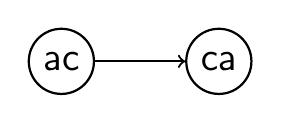
\begin{tikzpicture}[node distance=3cm, every loop/.style={},thick,main node/.style={circle,draw,font=\sffamily\Large}]

                \node[main node] (ac) {ac};
                \node[main node] at (2, 0) (ca) {ca};

                \path[->] (ac) edge[] node {} (ca);
            \end{tikzpicture}

            \caption{Exemplo da modelagem usada na solução}
            \label{fig:tanya}
        \end{figure}

        \sloppy Deve repetir-se tal procedimento para toda string $w \in \mathcal{C}$. Segue a modelagem completa, que chamaremos de $G$, do exemplo inicial ($\mathcal{C} = \{aca, aba, aba, cab, bac\}$):
       

        \begin{figure}[H]
            \centering
            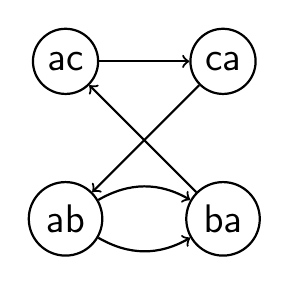
\begin{tikzpicture}[node distance=3cm, every loop/.style={},thick,main node/.style={circle,draw,font=\sffamily\Large}]

                \node[main node] (ac) {ac};
                \node[main node] at (2, 0) (ca) {ca};
                \node[main node] at(0, -2) (ab) {ab};
                \node[main node] at(2, -2) (ba) {ba};


                \path[->] (ac) edge[] node {} (ca);
                \path[->] (ab) edge[bend left] node {} (ba);
                \path[->] (ab) edge[bend right] node {} (ba);
                \path[->] (ca) edge[] node {} (ab);
                \path[->] (ba) edge[] node {} (ac);
            \end{tikzpicture}
        \end{figure}


        Cada arco criado na modelagem corresponde a uma string de $\mathcal{C}$, o arco entre $ac$ e $ca$, por exemplo, representa a string $aca$.
        A partir dessa correspondência podemos representar também um passeio, $P$, em $G$ como uma sequência de strings, $seq$, subconjunto de $\mathcal{C}$:

        O passeio $P = \{ba, ac, ca, ab\}$, por exemplo, percorre os arcos que correspondem à sequência $seq = \{bac, aca, cab\}$.

        Por sua vez, a partir de $seq$ é possível montar uma string $S$ que possua todas strings de $seq$ como substrings:

        \[seq = \{bac, aca, cab\} \rightarrow S = ``bacab'' \]

        Tal procedimento permite que, a partir de um passeio $P$ em $G$ construa-se uma string $S$ tal que:
        
        \begin{itemize}
            \item O tamanho de $S$ é igual ao número de arcos percorridos em $P$ mais 2;
            \item Se um arco $e$ é percorrido em $P$, então a string de $\mathcal{C}$ que $e$ representa será uma substring de $S$.
        \end{itemize}

        Como o problema pede que encontremos uma string de tamanho $n+2$ que possua todas strings de $\mathcal{C}$ como substrings, basta encontrar, se existir, uma trilha que percorra todo arco de $G$ uma única vez, isto é, uma trilha ou um circuito euleriano.

        Deste modo a solução do problema consiste em checar as propriedades necessárias para a existência de uma trilha euleriana, que são estabelecidas neste trabalho pelo corolário \ref{corollary-euler-digraph}.

        Se uma trilha ou circuito euleriano existir em $G$, podemos usar o algoritmo de Hierholzer para encontrar tal passeio.

        \section{Sereja and the Arrangement of Numbers}

        \hspace{0.55cm} URL do problema: \href{https://codeforces.com/problemset/problem/367/C}{https://codeforces.com/problemset/problem/367/C}

        URL da solução: \href{https://github.com/gafeol/competitive-programming/blob/master/ojs/cf/367/C.cpp}{https://github.com/gafeol/competitive-program\-ming\-/blob/master/ojs/cf/367/C.cpp}

        \textbf{Definição do problema}

        No enunciado do problema define-se uma sequência $s$ como \textbf{bonita} quando existe um inteiro $i$ para cada par de valores distintos $u$, $v$ pertencentes a $s$, tal que $s_i = u, s_{i+1} = v$ ou $s_i = v, s_{i+1} = u$.

        Em outras palavras, se uma sequência é bonita todo par de valores distintos pertencentes à essa sequência aparecem na mesma lado a lado ao menos uma vez.

        Define-se também um sistema de recompensas:
        para cada valor há uma recompensa positiva associada.
        A recompensa total de uma sequência é igual à soma das recompensas de seus valores distintos, ou seja, a recompensa não depende do número de vezes que cada valor aparece na sequência.

        O problema consiste então desenvolver um algoritmo que calcule a maior recompensa atingível para uma sequência bonita de tamanho $n$ que seja constituída apenas por valores definidos pela entrada. 

        A entrada do programa, portanto será dada pelos valores $n, m$ e por $m$ pares $q_i, w_i$, indicando que $q_i$ é um valor que pode ser utilizado e que possui recompensa $w_i$, garante-se que os valores de $q_i$ são distintos e que $w_i$ é positivo.

        Um exemplo de entrada para este problema é:

        \begin{align*}
            & 5 \text{ }4 & \text{Neste exemplo $n = 5$ e $m = 4$}\\
            & 1 \text{ }4 & \text{O primeiro valor é 1, e sua recompensa é 4}\\
            & 2 \text{ }3 & \text{Segue o valor 2, com recompensa 3}\\
            & 4 \text{ }2 & \text{Segue o valor 4, com recompensa 2}\\
            & 3 \text{ }10 &\text{Finalmente temos o valor 3, de recompensa 10}\\
        \end{align*}

        Para este exemplo, uma solução ótima é a sequência $1,2,3,1,1$, que é bonita e possui recompensa total igual a $17$. 
        Não existe uma sequência bonita que possua os quatro valores do exemplo.


        \textbf{Descrição da solução}

        Como todo valor possui uma recompensa positiva, a solução final deverá usar a maior quantidade de valores distintos que for possível.

        Começaremos discutindo um problema mais simples: Qual o tamanho da menor sequência bonita que utiliza $x$ valores distintos?

        Para resolver esse problema faremos uma modelagem do problema usando um grafo completo $K_x$, que possui $x$ vértices, onde cada vértice representa um valor distinto e cada aresta possui custo unitário.

        Todo passeio do grafo $K_x$ pode ser representado como uma sequência dos valores dos vértices do grafo, as sequências definidas como bonitas são aquelas que representam um passeio que percorre todas arestas do grafo $K_x$.

        Para facilitar a análise deste problema, assumiremos que pode existir em um passeio dois vértices de mesmo valor em sequência, mesmo sem haver um loop neste vértice, além disso, vamos assumir que os valores distintos são $1, 2, \dots, x$.

        Sendo assim, podemos interpretar uma sequência $s$ que possua apenas valores entre $1$ e $x$ como um passeio em $K_x$, os valores da sequência representam os vértices do grafo $K_x$, e dois valores adjacentes $u$ e $v$ representam que a aresta $uv$ está presente no passeio derivado de $s$. 
        
        Para que a sequência $s$ seja bonita, todo par de valores distintos $u, v$ deverá aparecer ao menos uma vez lado a lado, o que implica que o passeio derivado de $s$ deverá percorrer a aresta $uv$ ao menos uma vez.

        Concluimos então que um passeio derivado de uma sequência que seja bonita, deverá percorrer todas arestas do grafo $K_x$, sendo assim uma solução do problema do carteiro chinês para o mesmo.

        Voltamos assim à pergunta inicial, a menor sequência bonita que utiliza $x$ valores distintos, será aquela que representa uma solução ótima do problema do carteiro chinês para o grafo $K_x$, já que a solução que miniza o custo do PCC também minimizará o número de arestas percorridas, e portantom, o tamanho da sequência bonita.
 
        Vejamos agora alguns exemplos:

        \begin{figure}[H]
            \centering
            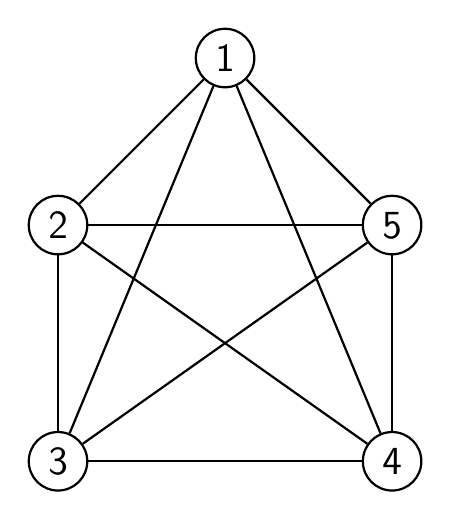
\begin{tikzpicture}[auto,node distance=3cm, every loop/.style={},thick,main node/.style={circle,draw,font=\sffamily\Large}]
                \node[main node] (1) {1};
                \node[main node] (2) [below left of=1] {2};
                \node[main node] (3) [below of=2] {3};
                \node[main node] (5) [below right of=1] {5};
                \node[main node] (4) [below of=5] {4};

                \path[every node/.style={font=\sffamily\small}]
                    (1) edge node [] {} (4)
                    (1) edge node [] {} (3)
                    (2) edge node [] {} (1)
                    (1) edge node [] {} (5)
                    (2) edge node [] {} (4)
                    (3) edge node [] {} (2)
                    (2) edge node [] {} (5)
                    (4) edge node [] {} (3)
                    (3) edge node [] {} (5)
                    (4) edge node [] {} (5)
                    ;
            \end{tikzpicture}
            \caption{Exemplo com $x=5$}
            \label{k5}
        \end{figure}

        Para $x=5$, o grafo induzido é o $K_5$, como representado na figura \ref{k5}.
        Como todos os vértices do $K_5$ possuem grau par, a solução ótima do Problema do Carteiro Chinês para este exemplo é também um circuito euleriano, como o seguinte:


        \[ P = \{1, 2, 3, 4, 5, 1, 3, 5, 2, 4, 1\} \]

        Como discutido anteriormente, $P$, além de solução do PCC é também uma sequência bonita que utiliza os $x$ valores definidos pelos vértices do grafo.
        
        Sendo assim, para utilizar $5$ valores distintos, é necessário ter uma sequência de tamanho no mínimo $11$, valor este que é igual a $1 + |E(K_5)| = 1 + 10 = 11$.

        Analisaremos agora outro exemplo, em que $x=4$, do qual se deriva o grafo $K_4$ representado na figura \ref{k4}.


        \begin{figure}[H]
            \centering
            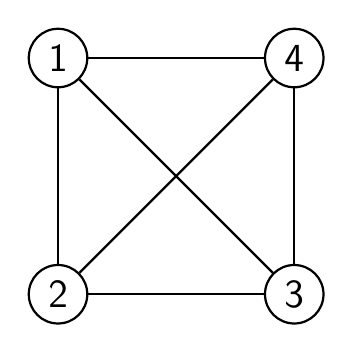
\begin{tikzpicture}[auto,node distance=3cm, every loop/.style={},thick,main node/.style={circle,draw,font=\sffamily\Large}]
                \node[main node] (1) {1};
                \node[main node] (2) [below of=1] {2};
                \node[main node] (4) [right of=1] {4};
                \node[main node] (3) [below of=4] {3};

                \path[every node/.style={font=\sffamily\small}]
                    (1) edge node {} (4)
                    (2) edge node {} (1)
                    (3) edge node {} (2)
                    (4) edge node {} (3)
                    (1) edge node {} (3)
                    (2) edge node {} (4)
                    ;
            \end{tikzpicture}
            \caption{Exemplo com $x=4$}
            \label{k4}
        \end{figure}


        Neste exemplo, todos os vértices de $K_4$ possuem grau ímpar, por isso, a primeira parte da solução do problema do carteiro chinês se baseia em duplicar algumas arestas do grafo, tornando-o um grafo euleriano.

        Como estamos tratando de um grafo completo, com arestas de custo unitário, não é necessário criar uma condensação do grafo $K_x$, e achar um emparelhamento perfeito de custo mínimo.
        Basta apenas criar uma duplicação de aresta entre todo par de vértices de índices $i$ e $i+1$ para todo índice $i$ ímpar, como representado na figura \ref{k4+} para o exemplo em questão.

        \begin{figure}[H]
            \centering
            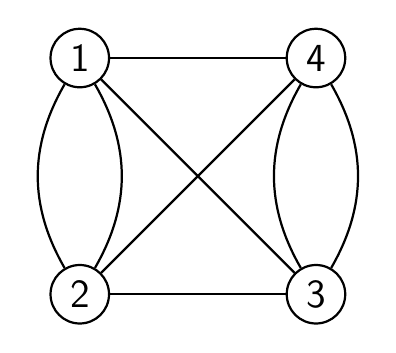
\begin{tikzpicture}[auto,node distance=3cm, every loop/.style={},thick,main node/.style={circle,draw,font=\sffamily\Large}]
                \node[main node] (1) {1};
                \node[main node] (2) [below of=1] {2};
                \node[main node] (4) [right of=1] {4};
                \node[main node] (3) [below of=4] {3};

                \path[every node/.style={font=\sffamily\small}]
                    (1) edge[] node {} (4)
                    (2) edge[bend right] node {} (1)
                    (4) edge[bend right] node {} (3)
                    (1) edge node {} (3)
                    (2) edge node {} (4)
                    (2) edge node {} (3)
                    (1) edge[bend right] node {} (2)
                    (3) edge[bend right] node {} (4)
                    ;
            \end{tikzpicture}
            \caption{$K_4$ com arestas duplicadas}
            \label{k4+}
        \end{figure}

        A partir do grafo euleriano criado, é possível encontrar o caminho euleriano $P$, que também é solução do PCC para o grafo $K_4$, e, finalmente, sequência bonita de tamanho mínimo que usa $4$ valores distintos.

        \[ P = \{1, 2, 3, 4, 1, 3, 4, 2, 1\} \]

        Sendo assim, o tamanho mínimo de uma sequência bonita que possui 4 valores distintos é $9$, valor este composto da seguinte forma: $1 + |E(K_4)| = 1 + 6 = 7$ somado ao número de arestas duplicadas $\frac{4}{2} = 2$.


        Podemos assim abstrair uma fórmula geral para o tamanho mínimo de uma sequência bonita $P$ que utilize $k$ valores distintos em sua composição:

        
        \[ |P|
             =  1 + \frac{k(k-1)}{2} + 
            \begin{cases} 
                0 & k \text{ ímpar} \\
                \frac{k}{2} & k \text{ par}
            \end{cases}
        \]

        Todo grafo completo com uma quantidade ímpar de vértices é euleriano, já que todos seus vértices possuem grau par, enquanto os grafos completos com quantidade par de vértices não são eulerianos. 
        Por isso a diferença na fórmula de $|P|$.

        A partir dessa fórmula fechada, é possível descobrir com uma busca binária, em complexidade $\mathcal{O}(\lg{n})$, qual o maior valor de $k$ tal que $|P| \leq n$.

        Encontrado tal valor $k$, o número máximo de valores distintos que a solução pode possuir para ser bonita, basta descobrir quais valores da entrada escolher para maximizar a recompensa.
        

        Se possuirmos na entrada uma quantidade de valores, $m$, tal que $m \leq k$, então a solução ótima será a soma das recompensas de todos valores, já que é possível encontrar uma sequência bonita que irá conter todos valores disponíveis.

        Do contrário, a solução consistirá em escolher os $k$ valores de maior recompensa disponíveis.
    Para encontrar tal valor, basta manter uma árvore de busca binária balanceada com as $k$ maiores recompensas dos valores disponíveis, o que custa tempo $\mathcal{O}(m\lg k) = \mathcal{O}(m\lg \sqrt{n})$.

        \section{Jogging Trails}

        \hspace{.55cm} URL do problema: \href{https://onlinejudge.org/index.php?option=com_onlinejudge&Itemid=8&page=show_problem&problem=1237}{https://onlinejudge.org/index.php?option=\-com\_\-onli\-ne\-judge\-\&Itemid\-=8\&page=show\_problem\&problem=1237}

        URL da solução: \href{https://github.com/gafeol/competitive-programming/blob/master/ojs/UVa/1237.cpp}{https://github.com/gafeol/\-compe\-titive-program\-ming\-/blob/master/ojs/UVa/1237.cpp}
        
        Neste problema devemos desenvolver um programa que calcula o custo de uma solução ótima para o problema do carteiro chinês em um grafo não direcionado de até 15 vértices com pesos nas arestas.

        Este problema é uma aplicação direta do problema descrito nesse trabalho. 
        Entretanto, em virtude do limite do número de vértices das instâncias, é possível resolver o problema de maneira mais simples.

        Um dos últimos passos do algoritmo que resolve o problema do carteiro chinês em grafos não direcionados descrito neste trabalho é realizar a condensação do grafo original usando os vértices de grau ímpar e posteriormente cosntruir o emparelhamento perfeito de custo mínimo usando o algoritmo de Edmonds.

        Uma alternativa viável para este problema é realizar a construção do emparelhamento perfeito usando, ao invés do algoritmo de Edmonds, um algoritmo de programação dinâmica:

         Para esta solução devemos memoizar o custo mínimo de emparelhamento perfeito para todo subconjunto de vértices do grafo condensado.

        Seja $K$ o grafo completo condensado, $S$ um subconjunto dos vértices de $K$, $dist$ uma função que retorna a distância entre dois vértices quaisquer de $K$ e $min\_cost_S$ o menor custo de emparelhamento perfeito do subconjunto $S$ de vértices, podemos definir a seguinte recorrência:

        \[
            min\_cost_S = 
            \begin{cases} 
                0 & S = \{ \} \\
                \min_{u, v \in S} min\_cost_{S - u - v} + dist(u, v) & \text{caso contrário}
            \end{cases}
        \]

        Para representar os subconjuntos de vértices pode-se utilizar uma bitmask.
        Como foi utilizado na implementação referenciada.
